\hypertarget{a00849}{}\section{V\+E\+N\+UE Guide}
\label{a00849}\index{VENUE Guide@{VENUE Guide}}
Details about using A\+AX plug-\/ins in V\+E\+N\+UE live sound systems. 

\hypertarget{a00849_aax_venue_guide_contents}{}\subsection{Contents}\label{a00849_aax_venue_guide_contents}
\begin{DoxyItemize}
\item \mbox{\hyperlink{a00849_aax_venue_guide__about_this_document}{About this document}} \item \mbox{\hyperlink{a00849_aax_venue_guide__overview}{Overview of V\+E\+N\+UE}} \item \mbox{\hyperlink{a00849_aax_venue_guide__systems}{V\+E\+N\+UE systems}} \item \mbox{\hyperlink{a00849_aax_venue_guide__environment}{Host environment}} \item \mbox{\hyperlink{a00849_aax_venue_guide__features}{A\+AX feature support and compatibility}} \item \mbox{\hyperlink{a00849_aax_venue_guide__installer}{V\+E\+N\+UE Plug-\/in installer specification}} \item \mbox{\hyperlink{a00849_aax_venue_guide__guidelines}{Additional plug-\/in guidelines}} \item \mbox{\hyperlink{a00849_aax_venue_guide__system_details}{System details}} \item \mbox{\hyperlink{a00849_aax_venue_guide__additional_information}{Additional Information}}\end{DoxyItemize}
 \hypertarget{a00849_aax_venue_guide__about_this_document}{}\subsection{About this document}\label{a00849_aax_venue_guide__about_this_document}
This guide discusses specific details related to creating A\+AX plug-\/ins which are compatible with Avid V\+E\+N\+UE systems.

This guide includes a general overview of the new V\+E\+N\+UE architecture as it pertains to plug-\/ins, a set of guidelines for developing compatible plug-\/ins, and details for creating full-\/featured plug-\/in installers for V\+E\+N\+UE.

\begin{DoxyNote}{Note}
Any reference in this document to \char`\"{}\+V\+E\+N\+U\+E\char`\"{} refers specifically to V\+E\+N\+UE $\vert$ S6L, and V\+E\+N\+UE $\vert$ S3L systems. Older V\+E\+N\+UE systems such as V\+E\+N\+UE Profile, D-\/\+Show, and S\+C48 are not compatible with A\+AX plug-\/ins and are not considered in this document.
\end{DoxyNote}


 \hypertarget{a00849_aax_venue_guide__overview}{}\subsection{Overview of V\+E\+N\+UE}\label{a00849_aax_venue_guide__overview}
 V\+E\+N\+UE is Avid\textquotesingle{}s product line aimed at live sound users. V\+E\+N\+UE systems are modular, with audio engine, control surface, console, I/O, and external G\+UI units.

 V\+E\+N\+UE offers plug-\/in racks to utilize the power of A\+AX D\+SP plug-\/ins. As virtual outboard racks inside the V\+E\+N\+UE system, the plug-\/in racks allow users to take their A\+AX D\+SP plug-\/ins out of the studio and into a live performance.

  Figure 1\+: The main V\+E\+N\+UE software interface

  Figure 2\+: V\+E\+N\+UE plug-\/in rack

 Using the V\+E\+N\+UE G\+UI, an operator is able to see thumbnails for each of the plug-\/ins in a plug-\/in rack. An operator can choose to zoom in on a plug-\/in from this rack view and, from there, graphically control the plug-\/in with the mouse, keyboard, or touch-\/screen. Only one plug-\/in interface can be displayed at a time in this mode.

  Figure 3\+: Plug-\/in zoom view



 \hypertarget{a00849_aax_venue_guide__systems}{}\subsection{V\+E\+N\+U\+E systems}\label{a00849_aax_venue_guide__systems}
 This section will provide a brief overview of Avid\textquotesingle{}s A\+A\+X-\/compatible V\+E\+N\+UE systems. For more information about the features, functionality, and use of these systems see the V\+E\+N\+UE user documentation.

\hypertarget{a00849_aax_venue_guide__systems__s6l}{}\subsubsection{V\+E\+N\+U\+E $\vert$ S6L}\label{a00849_aax_venue_guide__systems__s6l}
 V\+E\+N\+UE $\vert$ S6L is a modular system designed to take on the world\textquotesingle{}s most demanding tours and events with ease. Offering unprecedented processing capabilities -\/ with over 300 processing channels -\/ S6L delivers unrelenting performance and reliability through its advanced engine design and backs it up with modern touchscreen workflows and scalability to meet any challenge.

 The S6L engine contains dedicated H\+D\+X-\/powered D\+S\+Ps handling all plug-\/in processing and supports 64-\/bit A\+AX D\+SP plug-\/ins.

\hypertarget{a00849_aax_venue_guide__systems__s3l}{}\subsubsection{V\+E\+N\+U\+E $\vert$ S3\+L-\/X}\label{a00849_aax_venue_guide__systems__s3l}
 The V\+E\+N\+UE $\vert$ S3\+L-\/X System is a modular live sound solution including an H\+D\+X-\/powered processing engine, scalable remote I/O, and a E\+U\+C\+O\+N-\/enabled control surface.

 At the heart of the S3L system lies the E3 engine. The E3 runs Windows Embedded and a version of V\+E\+N\+UE software that can load A\+AX D\+SP plug-\/ins onto a built-\/in H\+DX platform. Accompanying the E3 engine is the \mbox{\hyperlink{a00833_subsubsection__avid_s3}{S3}} control surface and one or more Stage 16 remote I/O boxes.

 Most system parameters, including plug-\/ins, can be controlled using either the on-\/screen V\+E\+N\+UE software or directly via encoders on the S3 control surface. When being used as part of a V\+E\+N\+UE $\vert$ S3\+L-\/X system, the S3 control surface is divided into three main sections\+: A -\/ Channel Section The Channel section provides control of Input Channels, FX Returns, Output Channels, some channel parameters (such as Input Channel Gain and Aux Send levels), and channel banking. Channels are selected using the channel Select switches next to each fader.

 B -\/ Channel Control The eight Channel Control encoders provide control of processing functions for the currently selected Input or Output Channel. Inserted Dynamics and EQ plug-\/ins can be selected and adjusted in Channel Control.

 C -\/ Global Control The eight Global Control encoders provide control of system-\/wide parameters, including control of plug-\/ins. The Global Control encoders can be placed into Insert Mode, and can then be used to select and adjust any plug-\/ins.

  Figure 4\+: Main control sections on the S3 control surface

\hypertarget{a00849_aax_venue_guide__systems__s3l__using_channel_control}{}\paragraph{Using Channel Control}\label{a00849_aax_venue_guide__systems__s3l__using_channel_control}
 If a channel has an EQ, Comp/\+Lim, or Expander/\+Gate plug-\/in inserted on it, it can be controlled using the eight Channel Control encoders. The user can toggle between controlling the built-\/in Dynamics or EQ processors and the plug-\/in versions.

 Each Input and Output Channel has built-\/in EQ and Comp/\+Lim processors. Each Input Channel also has a built-\/in Expander/\+Gate. To adjust the built-\/in processors, the user selects a channel, assigns a processing function to Channel Control by pressing the corresponding encoder from the Channel Control main menu, then adjusts the available parameters.

  Figure 5\+: The Channel Control main menu

 See \mbox{\hyperlink{a00833_aax_page_table_guide_04_avid_center_section_page_tables_venue_s3l_mapping}{Center Section Parameter Mapping on V\+E\+N\+UE $\vert$ S3\+L-\/X}} for a description of how plug-\/in parameters are mapped to the S3L Channel Control encoders for EQ, Compressor/\+Limiter, and Expander/\+Gate plug-\/ins.



 \hypertarget{a00849_aax_venue_guide__environment}{}\subsection{Host environment}\label{a00849_aax_venue_guide__environment}
\hypertarget{a00849_aax_venue_guide__environment__audio_engine}{}\subsubsection{Audio engine}\label{a00849_aax_venue_guide__environment__audio_engine}
 The audio engine in V\+E\+N\+UE is based around Avid\textquotesingle{}s H\+DX technology. Each V\+E\+N\+UE S6L and S3L System contains a specialized H\+DX core card. For more information about H\+DX, see the \mbox{\hyperlink{a00832}{TI Guide}}. Because the V\+E\+N\+UE architecture is so similar to H\+DX, A\+AX D\+SP plug-\/ins are cross-\/compatible with V\+E\+N\+UE and most plug-\/ins will run seamlessly on V\+E\+N\+UE with little or no modification.

 Each V\+E\+N\+UE system operates at a single native sample rate. V\+E\+N\+UE supports multiple processing block sizes at this sample rate. Like in Pro Tools $\vert$ H\+DX systems, each D\+SP chip in the system will only be able to load plug-\/ins using a single block size; plug-\/ins which process using different block sizes cannot be allocated to the same D\+SP.

\hypertarget{a00849_aax_venue_guide__environment__dsp_resources}{}\subsubsection{Available D\+S\+P resources}\label{a00849_aax_venue_guide__environment__dsp_resources}
 The following information reflects plug-\/in processing abilities of V\+E\+N\+UE systems\+: 
\begin{DoxyItemize}
\item S3\+L-\/X 
\begin{DoxyItemize}
\item 4 TI C6727 D\+SP chips are available for plug-\/in processing 
\item 40 plug-\/in rack slots are available 
\end{DoxyItemize}
\item S6L 
\begin{DoxyItemize}
\item All H\+DX D\+SP cards are dedicated to plug-\/in processing; each H\+DX D\+SP card has 18 TI C6727 D\+SP Chips 
\item Depending on E6L engine type, 125 (E6\+L-\/144) or 200 (E6\+L-\/192) plug-\/in rack slots are available 
\end{DoxyItemize}
\end{DoxyItemize}

\hypertarget{a00849_aax_venue_guide__environment__operating_system}{}\subsubsection{Operating system}\label{a00849_aax_venue_guide__environment__operating_system}
 The core host software in a V\+E\+N\+UE system is built upon Windows Embedded 8. The installation used on V\+E\+N\+UE systems is a customized version of Windows 8 that includes only what is necessary for the V\+E\+N\+UE software.

 Core services from Windows 8 are available, such as the Win32 A\+PI, but some advanced services may not be available. Such services include M\+I\+DI, printing, video codec, .N\+ET, etc. If your code relies on advanced Win32 A\+P\+Is, or you are in doubt about specific A\+P\+Is, please contact Avid for more information.

 Using unavailable services may cause a plug-\/in to not load (e.\+g. if it attempts to link against D\+L\+Ls that aren\textquotesingle{}t included in the Windows Embedded 8 image) or to fail during run-\/time. Whenever possible, before using any advanced Win32 A\+PI, you should verify the availability of the service and/or handle the fact that the service might not be functional.

 See the \mbox{\hyperlink{a00849_aax_venue_guide__installer}{V\+E\+N\+UE Plug-\/in installer specification}} section for more information about ensuring that all required run-\/time components are available to your plug-\/in.

\hypertarget{a00849_aax_venue_guide__environment__display}{}\subsubsection{Display}\label{a00849_aax_venue_guide__environment__display}
 V\+E\+N\+UE S6L requires that plug-\/in windows be restricted to a certain size. If a plug-\/in exceeds this size, it will overlap V\+E\+N\+UE\textquotesingle{}s G\+UI and may possibly be truncated. The specifications are as follows\+: 
\begin{DoxyItemize}
\item S3\+L-\/X 
\begin{DoxyItemize}
\item Total G\+UI size\+: 1024 W x 768 H 
\item Max plug-\/in window size (w/o sidechain support)\+: 749 W x 617 H 
\item Max plug-\/in window size (with sidechain support)\+: 749 W x 565 H


\end{DoxyItemize}
\item S6L 
\begin{DoxyItemize}
\item Total G\+UI size\+: 1920 W x 1080 H 
\item Max plug-\/in window size (w/o sidechain support)\+: 1436 W x 855 H 
\item Max plug-\/in window size (with sidechain support)\+: 1436 W x 796 H


\end{DoxyItemize}
\end{DoxyItemize}

 V\+E\+N\+UE will dispatch a \mbox{\hyperlink{a00491_afab5ea2cfd731fc8f163b6caa685406ea74ab285136093261fd246572659f119c}{A\+A\+X\+\_\+e\+Notification\+Event\+\_\+\+Max\+View\+Size\+Changed}} notification indicating the maximum size for a plug-\/in\textquotesingle{}s G\+UI. Calls to \mbox{\hyperlink{a01889_ad750e9f0231c61ab32114276ee8cb5f7}{A\+A\+X\+\_\+\+I\+View\+Container\+::\+Set\+View\+Size()}} will fail with an error if the plug-\/in attempts to set its view size to a larger value than the system supports, though the plug-\/in\textquotesingle{}s initial G\+UI will be displayed (and possibly truncated) at its normal size before any resize requests are made.

 The actual hardware and graphical acceleration available in V\+E\+N\+UE systems is as follows\+: \tabulinesep=1mm
\begin{longtabu}spread 0pt [c]{*{3}{|X[-1]}|}
\hline
\cellcolor{\tableheadbgcolor}\textbf{ }&\cellcolor{\tableheadbgcolor}\textbf{ S3\+L-\/X }&\cellcolor{\tableheadbgcolor}\textbf{ S6L  }\\\cline{1-3}
\endfirsthead
\hline
\endfoot
\hline
\cellcolor{\tableheadbgcolor}\textbf{ }&\cellcolor{\tableheadbgcolor}\textbf{ S3\+L-\/X }&\cellcolor{\tableheadbgcolor}\textbf{ S6L  }\\\cline{1-3}
\endhead
\cellcolor{\tableheadbgcolor}\textbf{ C\+PU model }&Celeron P4500 &Core i5-\/2510E  \\\cline{1-3}
\cellcolor{\tableheadbgcolor}\textbf{ G\+PU model }&Intel HD Graphics &Intel HD Graphics 3000  \\\cline{1-3}
\cellcolor{\tableheadbgcolor}\textbf{ DirectX support }&10.\+1 &10.\+1  \\\cline{1-3}
\cellcolor{\tableheadbgcolor}\textbf{ Open\+GL support }&2.\+1 &3.\+1  \\\cline{1-3}
\cellcolor{\tableheadbgcolor}\textbf{ Open\+CL support }&None &None  \\\cline{1-3}
\cellcolor{\tableheadbgcolor}\textbf{ Shader model }&4 &4.\+1  \\\cline{1-3}
\end{longtabu}


\hypertarget{a00849_aax_venue_guide__environment__page_tables}{}\subsubsection{Page tables}\label{a00849_aax_venue_guide__environment__page_tables}
 
\begin{DoxyItemize}
\item V\+E\+N\+UE S3\+L-\/X uses {\ttfamily \textquotesingle{}Pc\+TL\textquotesingle{}} (Pro\+Control) page tables 
\item V\+E\+N\+UE S6L uses {\ttfamily \textquotesingle{}Av46\textquotesingle{}}, a E\+U\+C\+O\+N-\/style page table with a 4x6 knob cell configuration. 
\end{DoxyItemize}

 \begin{DoxyNote}{Note}
In S6L, the {\ttfamily \textquotesingle{}Fr\+TL\textquotesingle{}} (C$\vert$24) page table is used as a fallback when 4x6 is not available. This is only a temporary solution to support legacy plug-\/ins. All plug-\/ins targeting V\+E\+N\+UE S6L support must support the 4x6 knob cell layout and should not rely on this C$\vert$24 fallback behavior.
\end{DoxyNote}
Page table design guidelines Primary plug-\/in parameters should be located on the first page in the page tables for a surface. This is especially true for the 4x6 knob cell layout used by S6L. Users should not be required to navigate between pages for the majority of common operations.

 For more information about page tables, including additional guidelines for good page table design, see the \mbox{\hyperlink{a00833}{Page Table Guide}}.

\hypertarget{a00849_aax_venue_guide__environment__network}{}\subsubsection{Network communications}\label{a00849_aax_venue_guide__environment__network}
 Some plug-\/ins may require interaction with other devices in a network. V\+E\+N\+UE systems have two Gigabit Ethernet ports available\+: 
\begin{DoxyEnumerate}
\item {\bfseries{E\+Cx port}} Intended for connection of V\+NC Viewer to control the V\+E\+N\+UE system remotely. The IP address and network mask for this port are user-\/configurable in the V\+E\+N\+UE UI. 
\item {\bfseries{A\+VB port}} Intended for connection of all other V\+E\+N\+UE system components, as well as a computer running Pro Tools software. This port always uses link-\/local addressing. Because of A\+VB traffic, the effective bandwidth of this port is limited to 100 Mb/s. \begin{DoxyNote}{Note}
Plug-\/ins must not use a significant portion of the available bandwidth on the A\+VB port, since it will affect mission-\/critical control connections of a V\+E\+N\+UE system. 
\end{DoxyNote}

\end{DoxyEnumerate}

 Both S3\+L-\/X and S6L systems include the Apple Bonjour service. Plug-\/ins may use Bonjour for interfacing with other software in the network. Plug-\/ins must not install their own version of Bonjour or attempt to modify the Bonjour installation on the system.

\hypertarget{a00849_aax_venue_guide__environment__overview}{}\subsubsection{Host environment summary}\label{a00849_aax_venue_guide__environment__overview}
 \tabulinesep=1mm
\begin{longtabu}spread 0pt [c]{*{3}{|X[-1]}|}
\hline
\cellcolor{\tableheadbgcolor}\textbf{ }&\cellcolor{\tableheadbgcolor}\textbf{ S3\+L-\/X }&\cellcolor{\tableheadbgcolor}\textbf{ S6L  }\\\cline{1-3}
\endfirsthead
\hline
\endfoot
\hline
\cellcolor{\tableheadbgcolor}\textbf{ }&\cellcolor{\tableheadbgcolor}\textbf{ S3\+L-\/X }&\cellcolor{\tableheadbgcolor}\textbf{ S6L  }\\\cline{1-3}
\endhead
\cellcolor{\tableheadbgcolor}\textbf{ Operating System }&Windows Embedded 8 &Windows Embedded 8  \\\cline{1-3}
\cellcolor{\tableheadbgcolor}\textbf{ Sample Rate }&48 k\+Hz &96 k\+Hz  \\\cline{1-3}
\cellcolor{\tableheadbgcolor}\textbf{ Max G\+UI size }&749 W x 617 H (no sidechain)~\newline
749 W x 565 H (sidechain) &1436 W x 855 H (no sidechain)~\newline
1436 W x 796 H (sidechain)  \\\cline{1-3}
\cellcolor{\tableheadbgcolor}\textbf{ Page table }&{\ttfamily \textquotesingle{}Pc\+TL\textquotesingle{}} &{\ttfamily \textquotesingle{}Av46\textquotesingle{}}  \\\cline{1-3}
\end{longtabu}




 \hypertarget{a00849_aax_venue_guide__features}{}\subsection{A\+A\+X feature support and compatibility}\label{a00849_aax_venue_guide__features}
 V\+E\+N\+UE supports many of the same A\+AX features as Pro Tools. However, some features are not available in V\+E\+N\+UE, and other features are managed differently between the two applications. This section describes how V\+E\+N\+UE handles various optional A\+AX features.

\hypertarget{a00849_subsection__aax_venue_guide__features__processing}{}\subsubsection{Processing configurations}\label{a00849_subsection__aax_venue_guide__features__processing}
 Architectures V\+E\+N\+UE supports 64-\/bit A\+AX D\+SP plug-\/ins only. A\+AX Native and A\+AX Hybrid plug-\/ins are not supported. Plug-\/ins compiled for 32-\/bit processors are not supported, though they may be included in a V\+E\+N\+U\+E-\/compatible .aaxplugin bundle alongside the plug-\/in\textquotesingle{}s 64-\/bit binary.

 Stem formats 
\begin{DoxyItemize}
\item Mono plug-\/ins may be inserted as channel inserts on mono input strips and output busses. 
\item Stereo plug-\/ins can be inserted as channel inserts on stereo input strips and output busses. 
\item Greater-\/than-\/stereo formats are not supported by V\+E\+N\+UE 
\item Multi-\/mono processing is not supported; an operator must use the stereo version of a plug-\/in in stereo processing locations. 
\end{DoxyItemize}

 Width-\/changing plug-\/ins Width Changing plug-\/ins are not allowed as inserts except in mix busses. Unlike in Pro Tools, a plug-\/in cannot change the output stem format of a strip or bus by using a mono-\/to-\/stereo plug-\/in on a mono track.

 However, width-\/changing plug-\/ins are supported on output busses. For these, the outputs of the plug-\/in can either be routed back to an FX return or routed out to physical outputs. This functionality does not require any additional implementation specific to V\+E\+N\+UE.

\hypertarget{a00849_subsection__aax_venue_guide__features__presets}{}\subsubsection{Presets and automation}\label{a00849_subsection__aax_venue_guide__features__presets}
 Plug-\/\+In settings are persisted (saved \& restored) the same way for Show files, snapshots \& settings files, using a single method to extract settings and a single method to apply setting. The code uses the \char`\"{}chunk\char`\"{} A\+P\+Is. That\textquotesingle{}s similar to what Pro Tools does, except that for automation, V\+E\+N\+UE uses exclusively snapshots (that is, V\+E\+N\+UE does not record \& playback individual control changes).

 Many V\+E\+N\+UE snapshots users are known to store settings for every Plug-\/\+In in every snapshot (or almost). This causes performance issues because settings are often fairly slow to load, making a snapshot recall last too long (sometimes 30 seconds or more!) whereas users expect a snapshot recall to take instantly. However, extremely frequently, settings are not actually changing from a snapshot to the next one (that is, from one snapshot to the next one, the vast majority of Plug-\/\+Ins contain the same settings). To mitigate this, V\+E\+N\+UE calls \mbox{\hyperlink{a01669_a1e86f849e970c9998313fc7d451ccf85}{A\+A\+X\+\_\+\+I\+Effect\+Parameters\+::\+Compare\+Active\+Chunk()}} to determine whether a chunk from an incoming snapshot would result in any change to the plug-\/in\textquotesingle{}s current settings. If not, the new chunk will not be loaded onto the plug-\/in. This optimization is extremely effective, but requires that Plug-\/\+Ins implement the \mbox{\hyperlink{a01669_a1e86f849e970c9998313fc7d451ccf85}{Compare\+Active\+Chunk()}} method properly at any time (in particular regardless of whether the plug-\/in is visible or not). With V\+E\+N\+UE, you must implement this A\+PI very well or the Plug-\/\+In may not be controllable. This optimization will affect settings application when a show is loaded, when presets are loaded and when snapshots are recalled.

 All chunks are first compared one by one to the active chunks, until one is different or an error is returned. If any chunk compare fails (not equal or error returned), then all chunks are sent in sequence.

 As it is the basic method for plug-\/in settings manipulation, it is critical that plug-\/ins process chunks as accurately and efficiently as possible.

 Plug-\/\+In Chunks The size of a plug-\/in chunk cannot exceed 64KB in V\+E\+N\+UE. If a Plug-\/\+In requires more than 64KB of chunk data total (all chunk sizes added), settings for this plug-\/in won\textquotesingle{}t be persisted, snapshots won\textquotesingle{}t work for this plug-\/in and users won\textquotesingle{}t be able to load or save settings. If you can not meet this requirement, you should detect that you are running on V\+E\+N\+UE and not declared the process type as it won\textquotesingle{}t be usable.

\hypertarget{a00849_subsection__aax_venue_guide__features__unsupported}{}\subsubsection{Unsupported features}\label{a00849_subsection__aax_venue_guide__features__unsupported}
 The following A\+AX features are not supported by V\+E\+N\+UE. Plug-\/ins that require these features will not be compatible with V\+E\+N\+UE systems. If your plug-\/ins use these features for advanced functionality but not for basic operation then you should document this restriction for V\+E\+N\+UE users.

 
\begin{DoxyItemize}
\item Advanced audio routing  V\+E\+N\+UE does not support \mbox{\hyperlink{a00809}{Auxiliary Output Stems}} from plug-\/ins.

\begin{DoxyWarning}{Warning}
\mbox{\hyperlink{a00796}{Description callback}} calls to register auxiliary output stems will return an error code on V\+E\+N\+UE systems, indicating that the host will not provide audio buffers for auxiliary output stems during processing. A plug-\/in must not attempt to write data into auxiliary output stem buffers which have not been provided by the host!  
\end{DoxyWarning}

\item Transport interface  V\+E\+N\+UE operates entirely in real-\/time and does not contain a timeline of pre-\/recorded audio. Therefore V\+E\+N\+UE does not support the \mbox{\hyperlink{a01885}{A\+A\+X\+\_\+\+I\+Transport}} interface. V\+E\+N\+UE will return \mbox{\hyperlink{a00494_a5f8c7439f3a706c4f8315a9609811937a3b76994b32b97fcd56b19ef8032245df}{A\+A\+X\+\_\+\+E\+R\+R\+O\+R\+\_\+\+U\+N\+I\+M\+P\+L\+E\+M\+E\+N\+T\+ED}} to unsupported transport interface method calls.  
\item M\+I\+DI  V\+E\+N\+UE does not support M\+I\+DI routing to and from plug-\/in instances, and no \mbox{\hyperlink{a00806}{A\+AX M\+I\+DI features}} are supported by V\+E\+N\+UE.  
\end{DoxyItemize}



 \hypertarget{a00849_aax_venue_guide__installer}{}\subsection{V\+E\+N\+U\+E Plug-\/in installer specification}\label{a00849_aax_venue_guide__installer}
 To install plug-\/ins, the V\+E\+N\+UE software includes a simple installation interface. To install a plug-\/in, the operator simply plugs in a U\+SB Flash Drive with an installer for the plug-\/in and the plug-\/in will show up in an installer menu on the V\+E\+N\+UE interface (shown below).

 This menu will automatically list all the installable plug-\/ins on the drive. With the click of a button, the user can install the plug-\/ins onto his V\+E\+N\+UE system.

  Figure 6\+: The V\+E\+N\+UE plug-\/in installer tab

 For this custom installation to work properly, the plug-\/in installation U\+SB Key must follow a certain layout. This layout is designed to be as flexible and as expandable as possible, giving the developer many options while retaining the simplicity that makes V\+E\+N\+UE\textquotesingle{}s plug-\/in installation appealing to the user. This layout is also designed to coexist on a drive with a Pro Tools plug-\/in install. The following is a detailed description of how the file hierarchy should be laid out.

\hypertarget{a00849_subsection__aax_venue_guide__installer__overview}{}\subsubsection{Overview}\label{a00849_subsection__aax_venue_guide__installer__overview}
 The V\+E\+N\+UE Plug-\/\+In installer specification is an extension of an A\+AX plug-\/in bundle, i.\+e. of the {\itshape My\+Plug\+In}.aaxplugin folder.

 A standard .aaxplugin directory forms a basic, compatible plug-\/in installer for V\+E\+N\+UE. See \mbox{\hyperlink{a00801_commoninterface_formatspecification__aaxplugin_directory_structure}{.aaxplugin Directory Structure}} for more information about this folder.

 The following optional items can be added to the .aaxplugin folder to extend its functionality when used as a V\+E\+N\+UE plug-\/in installer\+: 
\begin{DoxyItemize}
\item License file that will need to be accepted by end user 
\item Pre-\/install action (either .bat script or executable or both) 
\item Post-\/install action (either .bat script or executable or both) 
\item Pre-\/uninstall action (either .bat script or executable or both) 
\item Post-\/uninstall action (either .bat script or executable or both) 
\item P\+A\+CE Eden installer to update the version pre-\/installed on the V\+E\+N\+UE system 
\item Factory presets 
\item Registry entries in a form of .reg files 
\item Program files to be placed in the system\textquotesingle{}s C\+:\textbackslash{}Program Files folder 
\item Plug-\/in thumbnails to be shown in the rack in V\+E\+N\+UE Software UI 
\end{DoxyItemize}

\hypertarget{a00849_subsection__aax_venue_guide__installer__format}{}\subsubsection{Directory structure}\label{a00849_subsection__aax_venue_guide__installer__format}
 Here is a layout of the optional elements in the .aaxplugin plug-\/in installer directory\+: 
\begin{DoxyItemize}
\item /\+Contents 
\begin{DoxyItemize}
\item {\itshape standard A\+AX plug-\/in contents} 
\end{DoxyItemize}
\item /\+Pace Eden 
\begin{DoxyItemize}
\item Setup.\+exe  
\item Setup.\+bat  
\item Version.\+txt  
\end{DoxyItemize}
\item /\+Program Files 
\begin{DoxyItemize}
\item ...  
\end{DoxyItemize}
\item /\+Thumbnails 
\begin{DoxyItemize}
\item {\itshape id1}.bmp (example\+: 424644204\+C41324131314\+C41.\+bmp)  
\item {\itshape id2}.bmp  
\end{DoxyItemize}
\item /\+License.rtf or License.\+txt  
\item /\+Install\+\_\+before.bat  
\item /\+Install\+\_\+before.exe  
\item /\+Install\+\_\+after.bat  
\item /\+Install\+\_\+after.exe  
\item /{\itshape Some\+Settings}.reg  
\item /\+Uninstall\+\_\+before.bat  
\item /\+Uninstall\+\_\+before.exe  
\item /\+Uninstall\+\_\+after.bat  
\item /\+Uninstall\+\_\+after.exe  
\end{DoxyItemize}

\hypertarget{a00849_subsection__aax_venue_guide__installer__optional_files}{}\subsubsection{Optional installer files}\label{a00849_subsection__aax_venue_guide__installer__optional_files}
\hypertarget{a00849_subsubsection__aax_venue_guide__installer__optional_files__license}{}\paragraph{License terms}\label{a00849_subsubsection__aax_venue_guide__installer__optional_files__license}
 A license stored as a file of either R\+TF or A\+S\+C\+II plain text format. The file must be located in the root folder of the installer. Depending on the text file format, the file name must be either {\itshape License.\+rtf} or {\itshape License.\+txt}.

\hypertarget{a00849_subsubsection__aax_venue_guide__installer__optional_files__registry}{}\paragraph{Registry entries}\label{a00849_subsubsection__aax_venue_guide__installer__optional_files__registry}
 Registry settings to be applied during installation need to be stored in .reg files in the root folder of installer. All such files must be of the Windows Registry format. Particular file names does not matter.

 Registry files are applied during plug-\/in installation.

 It is important to not alter any system settings or settings of other software installed.

 \begin{DoxyNote}{Note}
Changes in the registry are not reverted during the plugin uninstallation.
\end{DoxyNote}
\hypertarget{a00849_subsubsection__aax_venue_guide__installer__optional_files__program}{}\paragraph{Program files}\label{a00849_subsubsection__aax_venue_guide__installer__optional_files__program}
 Files under the {\itshape Program Files} subfolder in the plug-\/in installer will be copied to the system\textquotesingle{}s {\itshape C\+:\textbackslash{}Program Files} folder. All contents of the {\itshape Program Files} subfolder are copied as-\/is into {\itshape C\+:\textbackslash{}Program Files}, retaining the internal folder structure of nested directories.

 These changes are undone when the plug-\/in is uninstalled.

\hypertarget{a00849_subsubsection__aax_venue_guide__installer__optional_files__thumbnails}{}\paragraph{Plug-\/in thumbnails}\label{a00849_subsubsection__aax_venue_guide__installer__optional_files__thumbnails}
 V\+E\+N\+UE uses thumbnail images to display plug-\/in G\+U\+Is in the plug-\/in rack while the full-\/size plug-\/in G\+UI is hidden.

 If thumbnail images are not provided in the plug-\/in installer then V\+E\+N\+UE will display a generic thumbnail image for the plug-\/in until it has been focused in Zoom Mode in the V\+E\+N\+UE interface. In this case V\+E\+N\+UE will create and cache a thumbnail image for the plug-\/in G\+UI the first time that it is focused.

 The user may regenerate a thumbnail by right-\/clicking a rack with a plug-\/in and choosing \char`\"{}\+Recreate Thumbnail\char`\"{}.

 Including thumbnails in plug-\/in installers

 A separate thumbnail should be provided in the plug-\/in installer for each variant supported by the plug-\/in, i.\+e. each unique A\+AX D\+SP ID triad registered by the plug-\/in. Use the \char`\"{}\+Recreate Thumbnail\char`\"{} feature to create the initial versions of your plug-\/in thumbnail images. Package these thumbnail images into your plug-\/in installer in order to guarantee that thumbnail images will be available to users immediately upon installing the plug-\/in.

 Each thumbnail bitmap file is named after the following plug-\/in parameters\+: 
\begin{DoxyEnumerate}
\item \mbox{\hyperlink{a00662_a13e384f22825afd3db6d68395b79ce0da996465cca29a2a15291d1c788ac5728c}{A\+A\+X\+\_\+e\+Property\+\_\+\+Manufacturer\+ID}} 
\item \mbox{\hyperlink{a00662_a13e384f22825afd3db6d68395b79ce0da3a41fcdff5af1a4fd19dcbca7b1ba6f3}{A\+A\+X\+\_\+e\+Property\+\_\+\+Product\+ID}} 
\item \mbox{\hyperlink{a00662_a13e384f22825afd3db6d68395b79ce0da75f174df4efbeca86eaada126c1d9214}{A\+A\+X\+\_\+e\+Property\+\_\+\+Plug\+In\+I\+D\+\_\+\+TI}} 
\end{DoxyEnumerate}

 All of three are converted to hexadecimal representation and concatenated to form a file name that uniquely identifies a plug-\/in variant. For example, the Avid Channel Strip plug-\/in has a thumbnail file named 41564944 43685374 434D5469.bmp (no spaces).

 The \char`\"{}\+Recreate Thumbnail\char`\"{} feature in V\+E\+N\+UE will ensure that the generated thumbnail images use the correct file names, resolution, and image format.

\hypertarget{a00849_subsubsection__aax_venue_guide__installer__optional_files__actions}{}\paragraph{Actions}\label{a00849_subsubsection__aax_venue_guide__installer__optional_files__actions}
 A plug-\/in installer may define custom actions for the following cases\+: 
\begin{DoxyEnumerate}
\item Pre-\/install action -\/ executed when plug-\/in installation starts 
\item Post-\/install action -\/ executed when plug-\/in installation finishes 
\item Pre-\/uninstall action -\/ executed when plug-\/in uninstallation starts 
\item Post-\/uninstall action -\/ executed when plug-\/in uninstallation finishes 
\end{DoxyEnumerate}

 Each action is defined by either a .bat file or an Win32/64 executable file (.exe). Action files must be placed in the root folder of installer and use these file names\+: 
\begin{DoxyEnumerate}
\item Pre-\/install action -\/ {\itshape Install\+\_\+before.\+bat}, {\itshape Install\+\_\+before.\+exe} 
\item Post-\/install action -\/ {\itshape Install\+\_\+after.\+bat}, {\itshape Install\+\_\+after.\+exe} 
\item Pre-\/uninstall action -\/ {\itshape Uninstall\+\_\+before.\+bat}, {\itshape Uninstall\+\_\+before.\+exe} 
\item Post-\/uninstall action -\/ {\itshape Uninstall\+\_\+after.\+bat}, {\itshape Uninstall\+\_\+after.\+exe} 
\end{DoxyEnumerate}

 If both .exe and .bat files are present for a certain action, then both are executed, with the .bat file being run before the .exe.

 When executing an action, no exit code is tested. In order to report errors, the following needs to be done\+: 
\begin{DoxyEnumerate}
\item .bat files\+:

The following line should be used to report an error message from a script\+: {\ttfamily reg add H\+K\+CU\textbackslash{}Software\textbackslash{}Digidesign\textbackslash{}tmp /f /v Install\+Result /d \char`\"{}\+Error description\char`\"{}}  
\item .exe files\+:

The error message needs to be added to Windows registry as a R\+E\+G\+\_\+\+SZ value in {\itshape H\+K\+E\+Y\+\_\+\+C\+U\+R\+R\+E\+N\+T\+\_\+\+U\+S\+ER\textbackslash{}Software\textbackslash{}Digidesign\textbackslash{}tmp and named Install\+Result}.  
\end{DoxyEnumerate}

 The presence of the error message will abort a plug-\/in installation. Any error strings will be written to the V\+E\+N\+UE logs so that Avid support will be able to see them. Error strings from these actions are not shown to the user.

\hypertarget{a00849_subsubsection__aax_venue_guide__installer__optional_files__pace}{}\paragraph{P\+A\+C\+E software installer}\label{a00849_subsubsection__aax_venue_guide__installer__optional_files__pace}
 \begin{DoxyWarning}{Warning}
This functionality must not be used without prior approval from Avid. Before releasing {\bfseries{any}} V\+E\+N\+UE plug-\/in update with a bundled P\+A\+CE installer you must contact Avid to confirm that the bundled installer will not cause issues for deployed V\+E\+N\+UE systems.
\end{DoxyWarning}
V\+E\+N\+UE allows plug-\/ins to install updated version of P\+A\+CE i\+Lok software immediately after the plug-\/in installation. In general, Avid tries to provide the latest Pace software with each V\+E\+N\+UE software release and update. Therefore this step should not be necessary in most cases.

 The P\+A\+CE installer files must be located in {\itshape Pace Eden} subfolder of the installer. This folder must contain the following files\+: 
\begin{DoxyItemize}
\item {\itshape Version.\+txt} containing a version of the {\itshape L\+D\+Svc.\+exe} P\+A\+CE executable being installed. The version information must be in the form of {\itshape 1.\+2.\+3.\+4}  
\item {\itshape Setup.\+exe} -\/ the P\+A\+CE installer itself.  
\item (optional) {\itshape Setup.\+bat} containing an installation script. Usually used to run P\+A\+CE installer in a silent (no UI, no interaction) mode.  
\end{DoxyItemize}

 During installation, {\itshape Setup.\+bat}, if present, is run. Otherwise {\itshape Setup.\+exe} is executed with the following command line arguments\+:

 {\ttfamily Setup.\+exe /s /v"R\+E\+I\+N\+S\+T\+A\+L\+L\+M\+O\+DE=vamus R\+E\+B\+O\+OT=Really\+Suppress /qn"}

 If the version of installer is not higher than the version installed in system, the installation will not be performed.

 An OS reboot is prompted in V\+E\+N\+UE UI after P\+A\+CE was installed.

\hypertarget{a00849_subsection__aax_venue_guide__installer__use}{}\subsubsection{Using a V\+E\+N\+U\+E plug-\/in installer}\label{a00849_subsection__aax_venue_guide__installer__use}
 In order to install a plug-\/in to the V\+E\+N\+UE system, end user is expected to perform the following steps\+: 
\begin{DoxyEnumerate}
\item Download a V\+E\+N\+UE Plug-\/in Installer(s) in a form of archive (Zip is suggested). Is it ok to have multiple plug-\/ins in one archive as soon as each plug-\/in is in own V\+E\+N\+UE Plug-\/in Installer (i.\+e. in own .aaxplugin folder).  
\item Unpack archive and copy installers to U\+SB drive in the following way\+: 
\begin{DoxyEnumerate}
\item \char`\"{}\+A\+A\+X Plug-\/\+Ins\char`\"{} folder must be placed in the root of U\+SB drive.  
\item Each installer needs to be copied directly the \char`\"{}\+A\+A\+X Plug-\/\+Ins\char`\"{} folder. In the end, resulting folder structure will look like this\+:   
\end{DoxyEnumerate}
\item Install plug-\/ins in a way described in documentation of a particular V\+E\+N\+UE Software version.  
\end{DoxyEnumerate}





\hypertarget{a00849_aax_venue_guide__guidelines}{}\subsection{Additional plug-\/in guidelines}\label{a00849_aax_venue_guide__guidelines}
\hypertarget{a00849_subsection__aax_venue_guide__guidelines__reliability}{}\subsubsection{General Reliability and Fault Tolerance}\label{a00849_subsection__aax_venue_guide__guidelines__reliability}
 Since V\+E\+N\+UE is a more \char`\"{}mission critical\char`\"{} type of application where there is no room for error during a live show, additional precautions have to be taken with respect to reliability of its various components. We have built provisions in V\+E\+N\+UE to protect the system from catastrophic failure due to a plug-\/in crashing and bringing down the entire system. On top of this, extra care should be taken in developing stable software when targeting V\+E\+N\+UE as a platform.

 If a plug-\/in crashes, the user will be warned through a dialog. A crash brings down all plug-\/in processes, but audio keeps flowing through the console and through the D\+S\+Ps, including the plug-\/ins\textquotesingle{} D\+S\+Ps. All the effects continue to be effective, but their parameters can\textquotesingle{}t be accessed or modified anymore (the show goes on...).

 At this point, audio should be totally unaffected, even for the effect that caused the crash (assuming the crash took place in the host code, not the D\+SP code, of course). At the user\textquotesingle{}s discretion, all plug-\/ins will be bypassed or muted (depending on where they are used in the system), any dependencies on the plug-\/ ins\textquotesingle{} D\+S\+Ps will be removed, the plug-\/ins\textquotesingle{} D\+S\+Ps will be reset, and all the plug-\/ins will start again. When the rebuilding operation is complete, the user will be prompted to decide when he wishes the new plug-\/ins to be connected.

\hypertarget{a00849_subsection__aax_venue_guide__guidelines__dialogs}{}\subsubsection{Plug-\/\+In Dialogs}\label{a00849_subsection__aax_venue_guide__guidelines__dialogs}
 Plug-\/ins should avoid invoking dialog windows in V\+E\+N\+UE. We strongly suggest that any unnecessary dialog window your plug-\/in creates, whether at installation or instantiation, be removed. For V\+E\+N\+U\+E-\/only plug-\/ins, we strongly suggest to not make use of any dialog windows.

 Should you nevertheless need to make use of additional windows or dialogs, you need to make sure that they are front-\/most, so that they will not be hidden behind V\+E\+N\+UE\textquotesingle{}s G\+UI. The V\+E\+N\+UE software will try to force your windows to be front-\/most, but it is safer if your plug-\/in enforces this in the first place.

\hypertarget{a00849_subsection__aax_venue_guide__guidelines__help}{}\subsubsection{Online Help}\label{a00849_subsection__aax_venue_guide__guidelines__help}
 V\+E\+N\+UE currently doesn\textquotesingle{}t include any standardized help menu for plug-\/ins. We recommend that you use tooltips and other \char`\"{}live\char`\"{} help techniques similar to what plug-\/ins like Re\+Vibe II, Reverb One, and Smack! use to help the user. For instance, when a user clicks on the \char`\"{}\+Side-\/\+Chain E\+Q\char`\"{} label of the Smack! Plug-\/\+In, here\textquotesingle{}s what they see\+:

  Figure 7\+: Tooltip help in Avid\textquotesingle{}s Smack! plug-\/in

 One of the major benefits of this technique is that it is supported across platforms and will work the same in all \mbox{\hyperlink{a00852}{A\+AX}} hosts.



 \hypertarget{a00849_aax_venue_guide__system_details}{}\subsection{System details}\label{a00849_aax_venue_guide__system_details}
 \hypertarget{a00849_subsection__aax_venue_guide__system_details__dependencies}{}\subsubsection{External dependencies}\label{a00849_subsection__aax_venue_guide__system_details__dependencies}
 A\+AX plug-\/ins may rely on the presence of the following items in V\+E\+N\+UE systems\+:

 
\begin{DoxyItemize}
\item All V\+E\+N\+UE systems 
\begin{DoxyItemize}
\item Bonjour service and library

\begin{DoxyNote}{Note}
Plug-\/in installers are forbidden from installing over or modifying the pre-\/installed version of Bonjour on the V\+E\+N\+UE system.  
\end{DoxyNote}

\item VC 2005 x64 runtime 
\item VC 2008 x64 runtime 
\item VC 2010 x64 runtime 
\item VC 2012 x64 runtime 
\item VC 2013 x64 runtime 
\end{DoxyItemize}
\item S6L versions 5.\+7 and higher 
\begin{DoxyItemize}
\item VC 2015 x64 runtime 
\item VC 2017 x64 runtime 
\end{DoxyItemize}
\end{DoxyItemize}

 Because V\+E\+N\+UE does not execute standard software installers for plug-\/ins, Avid tries to keep VC runtime versions up to date relative to the moment of release of a particular V\+E\+N\+UE Software version.

 As of the time of this writing, Venue S3\+L-\/X systems are no longer receiving software updates and thus the S3L software will not be updated to include any additional system components beyond VC 2013.

 If you would like to provide compatibility with Venue host software which does not include your plug-\/in\textquotesingle{}s required runtime libraries then we recommend statically linking your plug-\/in to these runtime libraries.

\hypertarget{a00849_subsection__aax_venue_guide__system_details__environment_vars}{}\subsubsection{Environment variables}\label{a00849_subsection__aax_venue_guide__system_details__environment_vars}
 Both plug-\/in installers and actual plug-\/ins may rely on a presence of the following environment variables in a V\+E\+N\+UE system\+: 
\begin{DoxyItemize}
\item {\bfseries{{\ttfamily D\+A\+E\+P\+L\+U\+G\+I\+N\+S\+F\+O\+L\+D\+ER}}} -\/ is always set to the Installed Plug-\/ins location. Currently this is {\itshape C\+:\textbackslash{}Program Files\textbackslash{}Common Files\textbackslash{}Digidesign\textbackslash{}D\+AE\textbackslash{}Plug-\/\+Ins}. Final backslash is absent.  
\item {\bfseries{{\ttfamily J\+E\+X\+\_\+\+H\+O\+S\+T\+\_\+\+T\+Y\+PE}}} -\/ equals \char`\"{}venue\char`\"{}. If required, this may be used to provide a custom behavior of the plug-\/in when it\textquotesingle{}s run on V\+E\+N\+UE system.  
\end{DoxyItemize}

\hypertarget{a00849_subsection__aax_venue_guide__system_details__plugin_locations}{}\subsubsection{Plug-\/in file locations}\label{a00849_subsection__aax_venue_guide__system_details__plugin_locations}
 Installed Plug-\/\+Ins Located at {\itshape C\+:\textbackslash{}Program Files\textbackslash{}Common Files\textbackslash{}Digidesign\textbackslash{}D\+AE\textbackslash{}Plug-\/\+Ins}

 This folder is the only location used by V\+E\+N\+UE software to instantiate a plug-\/in.

 This location is different from the one used by Pro Tools and Media Composer for 64-\/bit \mbox{\hyperlink{a00852}{A\+AX}} plug-\/ins. The only way for a plug-\/in to appear at that location is to be installed from V\+E\+N\+UE Software\textquotesingle{}s \char`\"{}\+Options\char`\"{}$>$\char`\"{}\+Plug-\/\+Ins\char`\"{} page; standard plug-\/in installers will place the plug-\/in into a different directory.

 \begin{DoxyNote}{Note}
This location may change in future V\+E\+N\+UE software releases. Plug-\/ins should not make any assumptions about the install directory and should rely on the V\+E\+N\+UE plug-\/in installer to place them in the correct location.
\end{DoxyNote}
Plug-\/ins available for installation 
\begin{DoxyItemize}
\item Local\+: Located at {\itshape C\+:\textbackslash{}Program Files\textbackslash{}Common Files\textbackslash{}Avid\textbackslash{}Audio\textbackslash{}Plug-\/\+Ins}  
\item On U\+SB drive\+: Located at {\itshape (U\+SB drive letter)\+:\textbackslash{}\mbox{\hyperlink{a00852}{A\+AX}} Plug-\/\+Ins}  
\end{DoxyItemize}

 These locations can be chosen as sources for plug-\/in installation on V\+E\+N\+UE Software\textquotesingle{}s \char`\"{}\+Options\char`\"{}$>$\char`\"{}\+Plug-\/\+Ins\char`\"{} page.

 Cached plug-\/in installers Located at {\itshape D\+:\textbackslash{}D-\/\+Show\textbackslash{}Plug-\/\+In Installers}

 Contains copies of plug-\/in installers installed via V\+E\+N\+UE Software\textquotesingle{}s \char`\"{}\+Options\char`\"{}$>$\char`\"{}\+Plug-\/\+Ins\char`\"{} page.

 This location can be chosen as source for plug-\/in installation on V\+E\+N\+UE Software\textquotesingle{}s \char`\"{}\+Options\char`\"{}$>$\char`\"{}\+Plug-\/\+Ins\char`\"{} page under the name \char`\"{}\+Previous Installs\char`\"{}.

 Factory presets Located at {\itshape D\+:\textbackslash{}D-\/\+Show\textbackslash{}User Data\textbackslash{}Effect Presets\textbackslash{}Factory Presets}

 Contains preset files for plug-\/ins, as well as for certain V\+E\+N\+UE parameters. Presets are organized in folders.

 Each subfolder corresponds to a particular preset type. Plug-\/in presets are named after the plug-\/in\textquotesingle{}s name and the plug-\/in\textquotesingle{}s \mbox{\hyperlink{a01417_afbed1db12ae1f7cb3204dad3fd66070e}{A\+A\+X\+\_\+\+S\+Plug\+In\+Chunk\+Header\+::f\+Product\+ID}} value. For example, for an Avid Channel Strip plug-\/in the subfolder name is {\itshape Channel Strip \mbox{[}31313736\mbox{]}}, where \char`\"{}31313736\char`\"{} is an unsigned integer of the Channel Strip product ID.

 Contents of subfolders are .tfx files of plug-\/in presets. Each file name will be visible to end user as a preset name.

 Presets are copied into file location during a plug-\/in installation.

 Plug-\/in thumbnails Located at {\itshape C\+:\textbackslash{}Program Files\textbackslash{}Digidesign\textbackslash{}Plug-\/\+In Icons}

 Contains .bmp files of plug-\/in thumbnails generated by V\+E\+N\+UE Software as a result of saving current plug-\/in graphics into a bitmap. See \mbox{\hyperlink{a00849_subsubsection__aax_venue_guide__installer__optional_files__thumbnails}{Plug-\/in thumbnails}}.

\hypertarget{a00849_subsection__aax_venue_guide__system_details__plugin_installation}{}\subsubsection{Installation process}\label{a00849_subsection__aax_venue_guide__system_details__plugin_installation}
 \hypertarget{a00849_subsubsection__aax_venue_guide__system_details__plugin_installation__install}{}\paragraph{Plug-\/in installation}\label{a00849_subsubsection__aax_venue_guide__system_details__plugin_installation__install}
 These are the steps followed by V\+E\+N\+UE when installing a plug-\/in\+: 
\begin{DoxyEnumerate}
\item First, a V\+E\+N\+UE plug-\/in installer is cached. This is done by copying a plug-\/in from installation source to the Cached V\+E\+N\+UE Plug-\/\+In Installers location. All files are copied with an exception of the \char`\"{}\+Documentation\char`\"{} and \char`\"{}\+Pro Tools\char`\"{} folders.

All of the following steps are executed from the cached installer location, not from the original source location.  
\item The pre-\/install batch script (\char`\"{}\+Install\+\_\+before.\+bat\char`\"{}), if present, is executed. Execution assumes running the script without a console window.

\begin{DoxyNote}{Note}
The pre-\/install script must not contain any installation steps, since it\textquotesingle{}s executed before the plug-\/in license is accepted. In general, you should only use the pre-\/install script for pre-\/install checks.  
\end{DoxyNote}

\item The pre-\/install executable (\char`\"{}\+Install\+\_\+before.\+exe\char`\"{}), if present, is executed. Execution assumes running the executable without a console window.

\begin{DoxyNote}{Note}
The pre-\/install executable must not perform any installation steps, since it\textquotesingle{}s executed before the plug-\/in license is accepted. In general, you should only use the pre-\/install script for pre-\/install checks.  
\end{DoxyNote}

\item A license (\char`\"{}\+License.\+rtf\char`\"{} or \char`\"{}\+License.\+txt\char`\"{}), if present, is shown to the user. If \char`\"{}\+License.\+rtf\char`\"{} is not found, \char`\"{}\+License.\+txt\char`\"{} is used. A license, if present, must be accepted by user; otherwise installation will be aborted.  
\item All files of the V\+E\+N\+UE plug-\/in installer are copied to the system Installed Plug-\/\+Ins location, keeping the .aaxplugin folder structure. Failure to copy any of the items results in installation being aborted.  
\item If the plug-\/in installer contains a subfolder named \char`\"{}\+Program Files\char`\"{}, its contents are copied into \char`\"{}\+C\+:\textbackslash{}\textbackslash{}\+Program Files\char`\"{}. Failure to copy any of items results in installation being aborted.  
\item If the plug-\/in installer contains a subfolder named \char`\"{}\+Contents\textbackslash{}\textbackslash{}\+Factory Presets\char`\"{}, its contents are imported as plug-\/in presets. The \char`\"{}\+Factory Presets\char`\"{} folder must contain only valid plug-\/in .tfx preset files in an arbitrary folder structure. All preset files are read and copied into the system\textquotesingle{}s Factory Presets location.

\begin{DoxyNote}{Note}
It is important for a plug-\/in installer to contain only plug-\/in presets corresponding to plug-\/in being installed.  
\end{DoxyNote}

\item Plug-\/in thumbnails, if present, are copied from the \char`\"{}\+Thumbnails\char`\"{} subfolder of the installer to the system Plug-\/in Thumbnails location.  
\item Registry files, if any, are imported. Every file with .reg extension in the root of plug-\/in installer is treated as a Windows Registry file and gets imported by calling

{\ttfamily regedit /s \char`\"{}<file.\+reg>\char`\"{}}

No error checking is performed.  
\item The post-\/install batch script (\char`\"{}\+Install\+\_\+after.\+bat\char`\"{}), if present, is executed. Execution assumes running the script without a console window.  
\item The post-\/install executable (\char`\"{}\+Install\+\_\+after.\+exe\char`\"{}), if present, is executed. Execution assumes running the executable without a console window.  
\item The P\+A\+CE software installer, if present, is run. If the version of the installer is not higher than the version installed in system, the installation is not performed.

When installing multiple plug-\/ins at once, P\+A\+CE installation happens only after installing the final plug-\/in. V\+E\+N\+UE will use the P\+A\+CE installer with the highest available version among the installed plug-\/ins.  
\item Plug-\/in installation is considered successful.  
\end{DoxyEnumerate}

 If errors occur during installation, the following happens\+: 
\begin{DoxyEnumerate}
\item Plug-\/in files are removed from the disk (see \char`\"{}\+File removal\char`\"{} section for details). 
\item Cached plug-\/in installer is removed from the Cached V\+E\+N\+UE Plug-\/in Installers location. 
\end{DoxyEnumerate}

\hypertarget{a00849_subsubsection__aax_venue_guide__system_details__plugin_installation__removal}{}\paragraph{File removal}\label{a00849_subsubsection__aax_venue_guide__system_details__plugin_installation__removal}
 File removal happens either in case or plug-\/in uninstallation or in case of a failed installation cleanup.

 The following happens\+: 
\begin{DoxyEnumerate}
\item Plug-\/in files, as present in Cached V\+E\+N\+UE Plug-\/in Installers location, are removed from Installed Plug-\/\+Ins location.  
\item Plug-\/in Program Files files, as present in Cached V\+E\+N\+UE Plug-\/in Installers location, are removed from Installed Plug-\/\+Ins location.  
\end{DoxyEnumerate}

\hypertarget{a00849_subsubsection__aax_venue_guide__system_details__plugin_installation__uninstall}{}\paragraph{Plug-\/in uninstallation}\label{a00849_subsubsection__aax_venue_guide__system_details__plugin_installation__uninstall}
 Plug-\/in installation process is done by V\+E\+N\+UE Software. It removes a plug-\/in from the Installed Plugins location. Here\textquotesingle{}s a step by step process of uninstalling plug-\/in\+: 
\begin{DoxyEnumerate}
\item The pre-\/uninstall batch script (\char`\"{}\+Uninstall\+\_\+before.\+bat\char`\"{}), if present, is executed. Execution assumes running the script without a console window. NO return code is examined. Instead, a script is allowed to report an error string that will be visible to Avid support when examining V\+E\+N\+UE log files. The following line should be used to write an error message from a script\+:

{\ttfamily reg add H\+K\+CU\textbackslash{}Software\textbackslash{}Digidesign\textbackslash{}tmp /f /v Install\+Result /d \char`\"{}\+Error description\char`\"{}}

The presence of this string means an error has occurred and a plug-\/in uninstallation will abort.  
\item The pre-\/uninstall executable (\char`\"{}\+Uninstall\+\_\+before.\+exe\char`\"{}), if present, is executed. Execution assumes running the executable without a console window. NO return code is examined. Instead, an executable is allowed to report an error string that will be visible to Avid support when examining V\+E\+N\+UE log files. The error needs to be added to Windows registry as a {\ttfamily R\+E\+G\+\_\+\+SZ} value in {\itshape H\+K\+E\+Y\+\_\+\+C\+U\+R\+R\+E\+N\+T\+\_\+\+U\+S\+ER\textbackslash{}Software\textbackslash{}Digidesign\textbackslash{}tmp} and named {\itshape Install\+Result}. The presence of this string means an error has occurred and a plug-\/in uninstallation will abort.  
\item Plug-\/in files are removed. See \mbox{\hyperlink{a00849_subsubsection__aax_venue_guide__system_details__plugin_installation__removal}{File removal}} for details.  
\item The post-\/uninstall batch script (\char`\"{}\+Install\+\_\+after.\+bat\char`\"{}), if present, is executed. Execution assumes running the script without a console window. NO return code is examined. Instead, a script is allowed to report an error string that will be visible to Avid support when examining V\+E\+N\+UE log files. The following line should be used to write an error message from a script\+:

{\ttfamily reg add H\+K\+CU\textbackslash{}Software\textbackslash{}Digidesign\textbackslash{}tmp /f /v Install\+Result /d \char`\"{}\+Error description\char`\"{}}

The presence of this string means an error has occurred and a plug-\/in uninstallation will abort.  
\item The post-\/uninstall executable (\char`\"{}\+Install\+\_\+after.\+exe\char`\"{}), if present, is executed. Execution assumes running the executable without a console window. NO return code is examined. Instead, an executable is allowed to report an error string that will be visible to Avid support when examining V\+E\+N\+UE log files. The error needs to be added to Windows registry as a {\ttfamily R\+E\+G\+\_\+\+SZ} value in {\itshape H\+K\+E\+Y\+\_\+\+C\+U\+R\+R\+E\+N\+T\+\_\+\+U\+S\+ER\textbackslash{}Software\textbackslash{}Digidesign\textbackslash{}tmp} and named {\itshape Install\+Result}. The presence of this string means an error has occurred and a plug-\/in uninstallation will abort.  
\item Plug-\/in removal is complete.  
\end{DoxyEnumerate}

Please note that plug-\/in being uninstalled is not being removed from the cache. Removal from the Cached V\+E\+N\+UE Plug-\/in Installers is possible for plug-\/ins being not installed. In order to accomplish this, end user needs to go to V\+E\+N\+UE Software\textquotesingle{}s \char`\"{}\+Options\char`\"{}$>$\char`\"{}\+Plug-\/\+Ins\char`\"{} page, right click on cached installer, and choose \char`\"{}\+Delete $<$em$>$plug-\/in name$<$/em$>$\char`\"{}.



 \hypertarget{a00849_aax_venue_guide__additional_information}{}\subsection{Additional Information}\label{a00849_aax_venue_guide__additional_information}
 \hypertarget{a00849_subsection__aax_venue_guide__additional_information__metering}{}\subsubsection{Metering}\label{a00849_subsection__aax_venue_guide__additional_information__metering}
 For metering displays, V\+E\+N\+UE uses dB units referenced to V\+E\+N\+UE\textquotesingle{}s nominal operating level of +4d\+Bu. A signal at the nominal level in V\+E\+N\+UE (i.\+e. registers 0dB on the V\+E\+N\+UE meters) will, at unity gain, generate a +4d\+Bu analog output signal (-\/20d\+B\+FS digital output signal).

 As a result, a signal that registers +20dB on the V\+E\+N\+UE meters will register 0d\+B\+FS on the plug-\/in meters. A signal at 0 dB in V\+E\+N\+UE will be -\/20d\+B\+FS in the plug-\/in.

 To map between d\+B\+FS units used in plug-\/ins and dB units used in V\+E\+N\+UE the operator simply needs to add 20 to any plug-\/in d\+B\+FS value.

 Collaboration diagram for V\+E\+N\+UE Guide\+:
\nopagebreak
\begin{figure}[H]
\begin{center}
\leavevmode
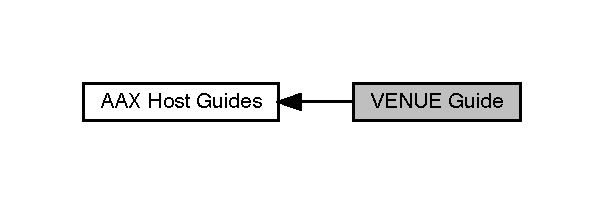
\includegraphics[width=290pt]{a00849}
\end{center}
\end{figure}
